\section{Abstände}
%


	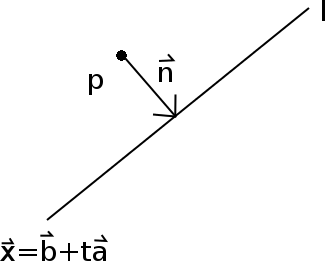
\includegraphics[width=0.2\textwidth]{mainmatter/chapter1/pics/gerade.png}
%
\begin{itemize}
	\item Abstand von $p$ zur Gerade $\vec{b} + \mathbb{R}\vec{a}$ ist $\frac{\vert 
	det(p-b,a)\vert}{\Vert\vec{a}\Vert}$ 
	\item Abstand von $p$ zur Gerade $<n,x>=c$ ist $ \frac{\vert <n,p>-c\vert}{\Vert 
	\vec{n}\Vert}$, unabhängig von Wahl von $\vec{n}$
\end{itemize}
%
%
%
\subsubsection{Beweis:}
\begin{itemize}
	\item will ausrechnen $\Vert\vec{x}-\vec{p}\Vert$ minimal, $x \in l$\\
	$det(x-p,a)=det(b-p,a)$\\
	$det(x-p,a)=\Vert x-p\Vert\mathop{\underbrace{\sin\measuredangle(b-
	p,a)}}\limits_{=1\text{ wenn }\vec{x}-\vec{p}\perp\vec{a}}\Vert a\Vert$ also $x-p 	
	\perp a$\\
	$\vec{n}\perp\vec{a} \quad p+\mathbb{R}n \cap b +\mathbb{R}a$\\
	$\Rightarrow \Vert x-p,a\Vert=\frac{det(x-p,a)}{\Vert\vec{a}\Vert}$also $x-p\perp a$
	
	\item $<\vec{n},\vec{x}>=c=<\vec{n},b> \, \frac{<n,p>-<n,b>}{\Vert\vec{n}\Vert}$\\
	Nimm $\vec{n}=\begin{pmatrix} -a_{2} \\ a_{1} \end{pmatrix}$\\
	$\frac{\vert det(\vec{p}-b,a)\vert}{\Vert\vec{a}\Vert} \mathop{=}\limits^{det(\vec{a},
	\vec{b})
	=<a^{\perp},>}\frac{\vert <p-b,\vec{n}> \vert}{\Vert\vec{n}\Vert}=\frac{\vert<p,n>-
	c\vert}{\Vert\vec{n}\Vert}$
\end{itemize}
%
%
%
\subsubsection{Satz:}
\begin{enumerate}
	\item $\vec{a},\vec{b}\in\mathbb{R}^{2}$: Punkte der Winkelhalbierenden  
	$\mathbb{R}(\Vert b\Vert a+\Vert a\Vert b)$ haben den gleichen Abstand zu 
	$\vec{a}$ und $\vec{b}$. \\
	(beachte: $\mathbb{R}\frac{1}{2}(\frac{\vec{a}}{\Vert a\Vert}+\frac{\vec{b}}{\Vert 
	b\Vert})=\mathbb{R}(\Vert \vec{b}\Vert\vec{a}+\vec{b}\Vert\vec{a}\Vert)$)
	\item Die drei Winkelhalbierenden eines Dreiecks gehen durch einen Punkt = 
	Inkreismittelpunkt.
\end{enumerate}
%
%
%
\subsubsection{Beweis:}
\begin{enumerate}
	\item $\vec{v}=\Vert\vec{b}\Vert\vec{a}+\Vert\vec{a}\Vert\vec{b}, \, \lambda >0$\\
	Abstand von $\lambda\vec{v}$ zu $\mathbb{R}a$ und $\mathbb{R}b:$\\
	$\frac{det(\lambda v,\vec{a})}{\Vert\vec{a}\Vert}=\lambda \vert det(\vec{a},
	\vec{b})\vert = \frac{\vert det(\lambda \vec{v},\vec{b}\vert}{\Vert\vec{b}\Vert}$
	%
	%Grafik einfügen
	%
	\item $C = \Vert b-a\Vert, B=\Vert c-a \Vert, A=\Vert b-c \Vert$\\
	Winkelhalbierende durch $\vec{a}: \vec{a}+\mathbb{R}(C(c-a)+B(b-a))$\\
	Parameter $\frac{1}{A+B+C}:\frac{1}{A+B+C}(Aa+Bb+Cc)$\\
	Symmetrie $\Rightarrow$ Schnittpunkt
\end{enumerate}
%
%
%
\subsubsection{Satz:}
$l$ und $m$ zwei verschiedene Geraden
\begin{enumerate}
	\item $l$ $||$ $m: \{P|d(P,l)=d(P,m)\}$ ist Gerade parallel zu l und m 
	\item $l \cap m=\{*\}$ $m: \{P|d(P,l)=d(P,m)\}$ ist Vereinigung zweier zueinander 
	senkrechter Geraden
\end{enumerate}
%
%
%
\subsubsection{Beweis:}
\begin{enumerate}
	\item $l:ax+by=c $ und $  m:ax+by=d$\\
	Abstand $\begin{pmatrix} x \\ y\end{pmatrix}$ zu $l: \frac{1}{\sqrt{a^{2}+b^{2}}} |
	ax+by-c|$\\
	bzw.: $\frac{1}{\sqrt{a^{2}+b^{2}}}|ax+by-d|$\\
	$\Rightarrow ax+by-c=\pm(ax+by-d)$\\
	$\Rightarrow 2ax+2by=c+d \Rightarrow ax+by=\frac{1}{2} c+d$
	\item $ax+by=c \,$ o.E. $a^{2}+b^{2}=1=e^{2}+f^{2}$\\
	$ex+fy=g$\\
	$|ax+by-c|=|ex+fy-g|$\\
	$\Leftrightarrow ax+by-c=\pm(ex+fy-g)$\\
	$\Rightarrow (a+e)x+(b+f)y=c+g \vee (a-e)x+(b-f)y=c-g \leadsto$ die beiden 
	Geraden. Noch z.z.: orthogonal\\
	$\begin{pmatrix} a+e \\ b+f \end{pmatrix} \begin{pmatrix} a-e \\ b-f \end{pmatrix} = 
	a^{2}+b^{2}-e^{2}-f^{2}=1-1=0$
\end{enumerate}